\documentclass[a4paper,12pt]{article}

\title{Physics 30 \\ Momentum and Impulse}
\author{Jad Chehimi}

% document setup
\renewcommand{\familydefault}{\sfdefault}
\linespread{1.25}
\usepackage[margin=1in]{geometry}
\usepackage{setspace}
\usepackage{enumitem}
\setlist{nosep}
\usepackage{color,soul}
\setcounter{secnumdepth}{0}

% tools
\usepackage[hidelinks]{hyperref}
\usepackage{float}
%% images
\usepackage{graphicx}
\graphicspath{ {./images/} }
%% science
\usepackage{siunitx}
\usepackage{physics}

\begin{document}
%%\sisetup{exponent-product = \cdot, output-decimal-marker = {,}, per-mode = fraction}
\maketitle


% temp
\begin{center}
\Huge
Unfinished!
\normalsize
\end{center}
% temp

\tableofcontents

\pagebreak

\section{Review}
\subsection{Scalar v/s Vector Quantity}
\begin{itemize}
    \item{\textbf{Scalar} = Magnitude (size) only}
    \item{\textbf{Vector} = Magnitude (size) AND direction}
\end{itemize}

\subsection{Sig Digs}
\subsubsection{Multiplication \& Division}
Least number of sig digs in numbers provided by question.

\subsubsection{Addition \& Subtraction}
p

\subsection{Unit Analysis}
\subsubsection{km/h to m/s}
$$\SI{100}{\km/\hour} \times \frac{\SI{1000}{\m}}{\SI{1}{\km}} \times \frac{\SI{1}{\hour}}{\SI{3600}{\second}}$$

\subsection{Proportional}
\Large $$a \propto b$$ \normalsize
If a variable is proportional to the other, increasing one will increase the other, same with decreasing.
\Large $$a \propto \frac{1}{b}$$ \normalsize
If a variable is inversely proportional to the other, increasing one will decrease the other, and vice versa.
\begin{figure}[H]
    \centering
    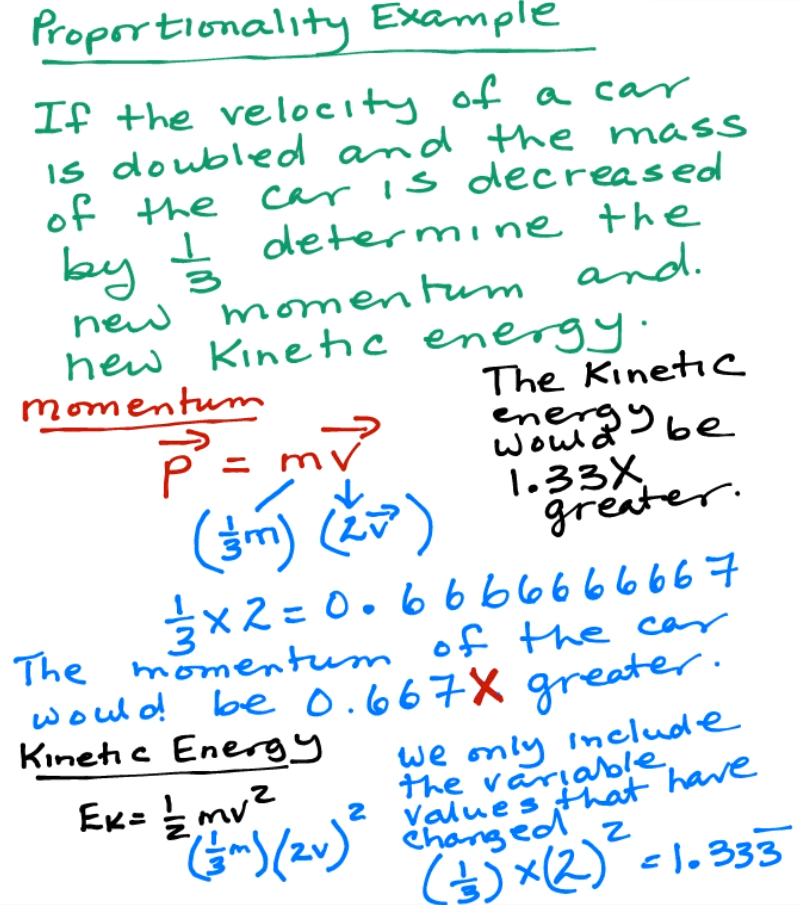
\includegraphics[width=0.50\textwidth]{q-prop}
    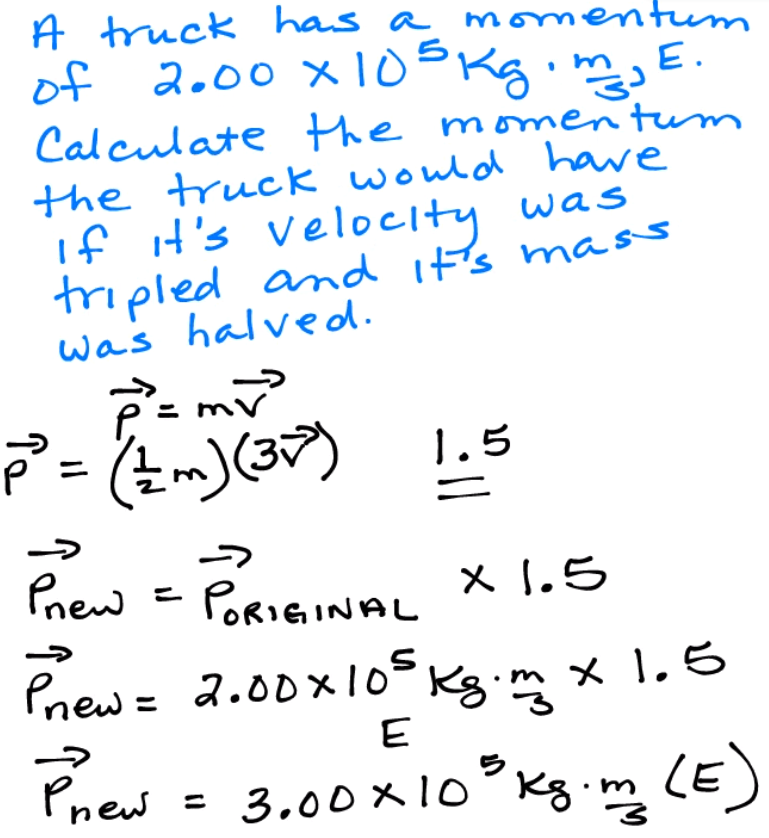
\includegraphics[width=0.50\textwidth]{q-prop-2}
\end{figure}

\subsection{Conventions}
\subsubsection{Signs}
\begin{itemize}
    \item{$+$ positive: right, up, north, east}
    \item{$-$ negative: left, down, south, west}
\end{itemize}

\subsubsection{Direction}
\begin{figure}[H]
    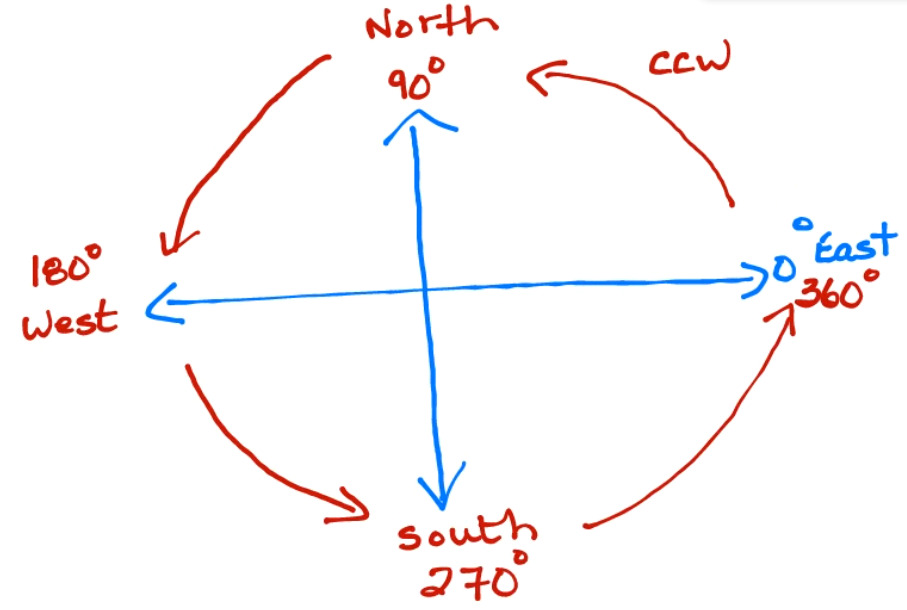
\includegraphics[width=0.75\textwidth]{direction}
\end{figure}

\subsubsection{Uniform Velocity}
$$v = \frac{d}{t}$$
Uniform = constant: velocity does not change over time.

\subsubsection{Formula Review}
$$g = \SI{9.81}{\m/\s^2}$$

$$\sum{E_{top}} = \sum{E_{bottom}}$$
$$E_p + E_k = E_p + E_k$$

$$\textrm{Newton's 2nd Law (Force, in N)} = \vec{F} = m\vec{a}$$
$$\textrm{Weight (N)} = \vec{F_g} = m\vec{g}$$

\pagebreak

\section{Momentum}
\Large $$\vec{p} = m\vec{v}$$ \normalsize

\begin{itemize}
    \item{$\vec{p}$ = momentum, product of mass and velocity\\vector quantity, $\si{\kg\cdot\m/\s}$}
    \item{$m$ = mass\\scalar quantity, $\si{\kg}$}
    \item{$\vec{v}$ = velocity\\vector quantity, $\si{\m/\s}$}
\end{itemize}
\Large
$$\vec{p} \propto m$$
$$\vec{p} \propto \vec{v}$$
\normalsize

\subsection{Examples}
\begin{figure}[H]
    \centering
    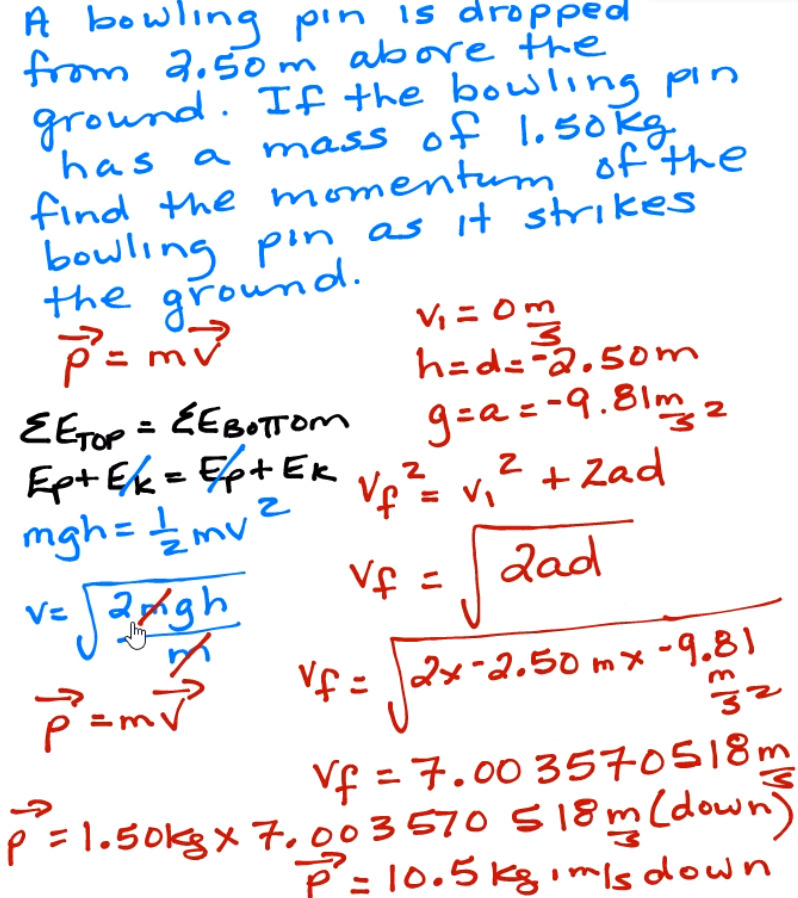
\includegraphics[width=0.75\textwidth]{q-mom}
\end{figure}
\begin{figure}[H]
    \centering
    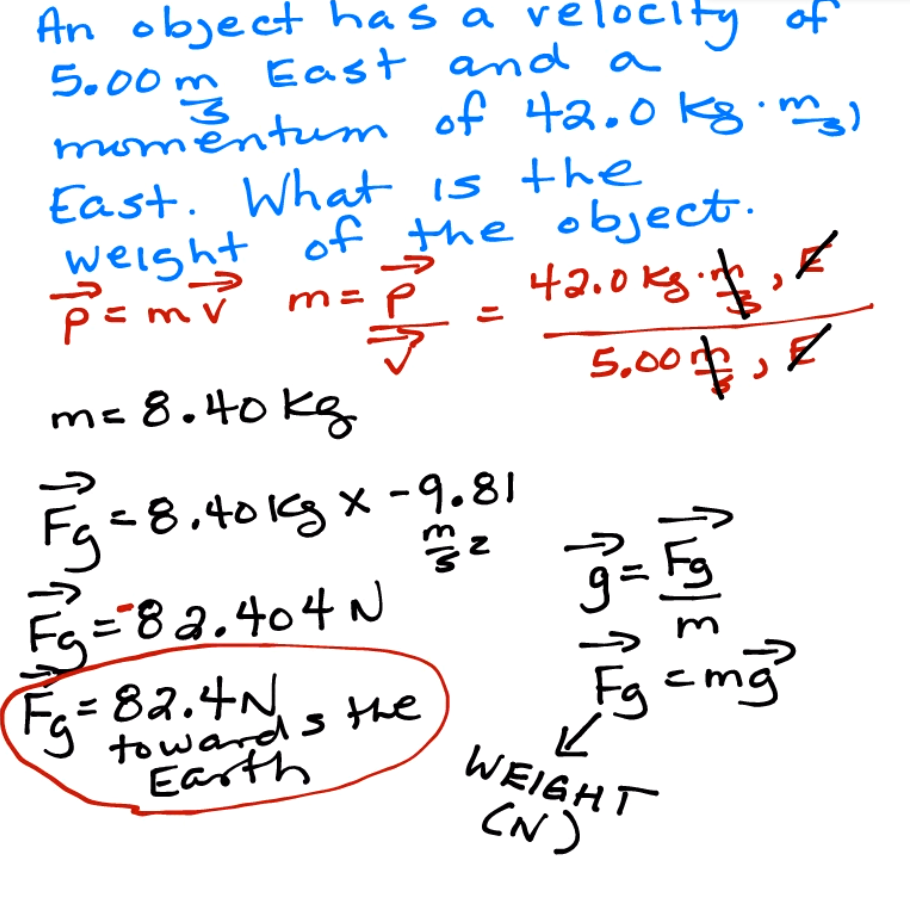
\includegraphics[width=0.75\textwidth]{q-mom-2}
\end{figure}
\begin{figure}[H]
    \centering
    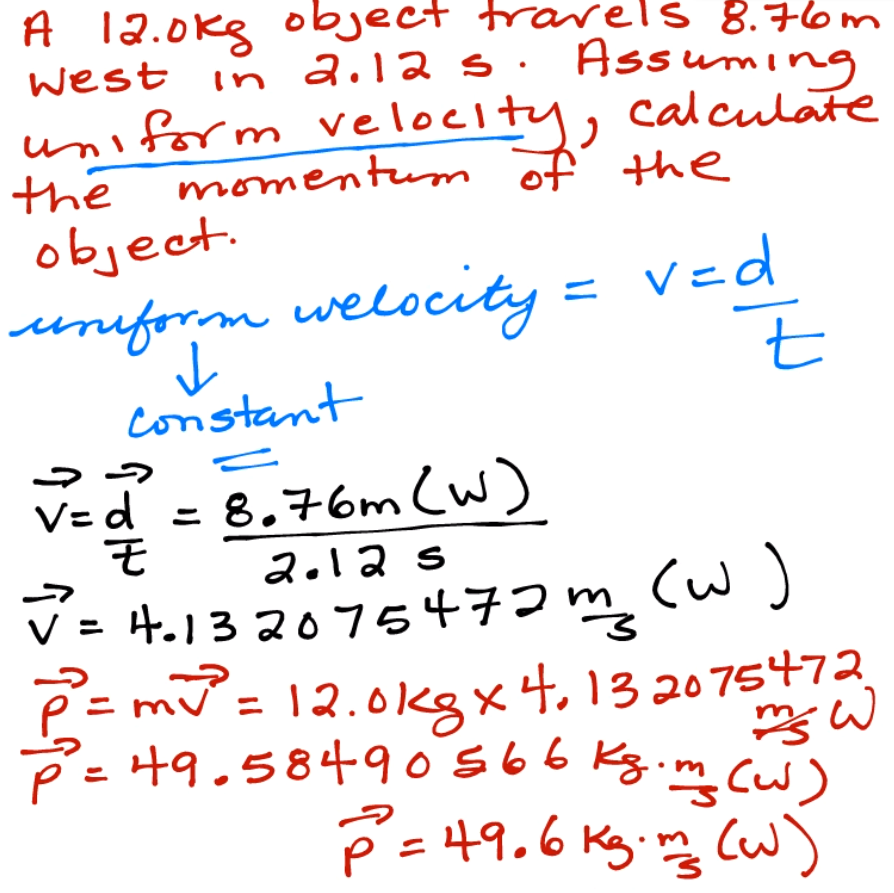
\includegraphics[width=0.75\textwidth]{q-mom-3}
\end{figure}

\section{Impulse}
\Large $$\Delta\vec{p} = \vec{p}_f - \vec{p}_i$$ \normalsize

Impulse is change in momentum; a \hl{force applied} to an object will \hl{change its momentum}.

\subsection{Formula}
\Large $$\Delta\vec{p} = \vec{F}\Delta{t} = m\Delta{\vec{v}}$$ \normalsize
$$\si{\kg\cdot\m/\s} = \si{\newton\cdot\s} = \si{\kg\cdot\m/\s}$$

Can be reorganized into Newton's 2nd law.
$$\vec{F} = \frac{m\Delta\vec{v}}{\Delta{t}} = m\Delta{a}$$
$$\vec{F} \propto \frac{1}{\Delta{t}}$$
Force is inversely proportional to time; a large force will be in small time (swift execution), a small force will be over large time.

\begin{figure}[H]
    \centering
    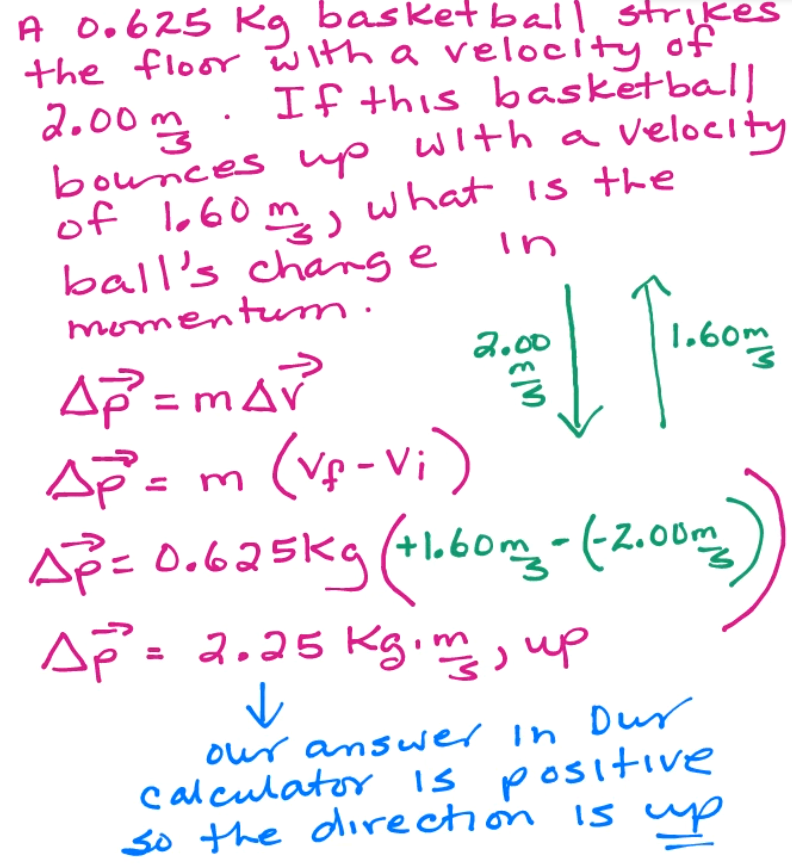
\includegraphics[width=0.7\textwidth]{q-imp}
\end{figure}
\begin{figure}[H]
    \centering
    \caption{A frictionless disc of mass \SI{0.500}{\kg} is moving in a straight line across an air table top at a speed of \SI{2.40}{\m/\s} when the disc bumps into an elastic band stretched between two fixed posts. If the elastic band exerts an opposing force of \SI{1.40}{\N} on the disc for \SI{1.50}{\s}, calculate the final velocity of the disc.}
    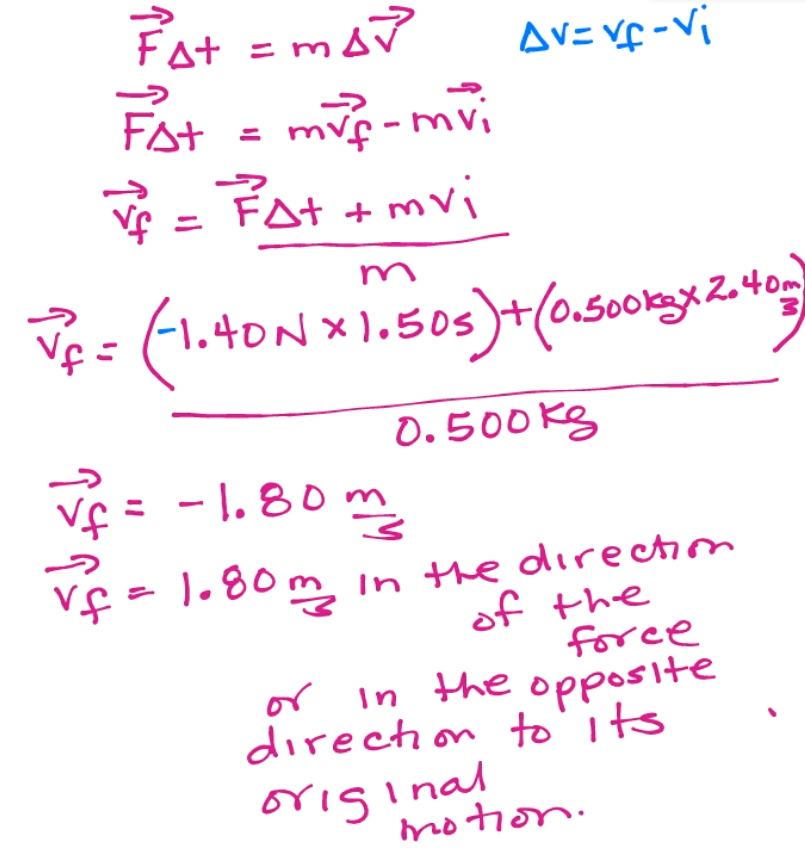
\includegraphics[width=0.8\textwidth]{q-imp-2}
\end{figure}

\end{document}
